\section{Architecture Integration}

\subsection{Model Support}

\begin{table}[H]
\centering
\small
\begin{tabular}{llllll}
\toprule
\textbf{Model} & \textbf{Attention class} & \textbf{Nested?} & \textbf{RoPE?} & \textbf{GQA?} & \textbf{Conv1D?} \\
\midrule
DistilBERT & \texttt{MultiHeadSelfAttention} & No & No & No & No \\
RoBERTa & \texttt{BertSelfAttention} & Yes & No & No & No \\
GPT-2 & \texttt{GPT2Attention} & No & No & No & Yes \\
Qwen3.5 & \texttt{Qwen3Attention} & No & Yes & Yes & No \\
\bottomrule
\end{tabular}
\end{table}

\subsection{Weight Transfer}

\texttt{copy\_weights} extracts weights via a five-tier strategy:

\subsubsection{Tier 1: UniversalAdapter}

\begin{lstlisting}
for proj in ["q", "k", "v", "o"]:
    try:
        w, b = UniversalAdapter.get\_weight\_bias(src, proj)
        if w is not None:
            extracted[proj] = (w, b)
    except Exception as e:
        logger.debug(f"UniversalAdapter failed for {proj}: {e}")
\end{lstlisting}

Note: failures are \textbf{logged and continued}, not raised.

\subsubsection{Tier 2: GPT-2 Conv1D}

\begin{lstlisting}
weight = src.c\_attn.weight.data
if weight.shape[1] == 3 * hidden\_size:
    weight = weight.t()
q\_w, k\_w, v\_w = weight.chunk(3, dim=0)
\end{lstlisting}

\subsubsection{Tier 3: RoBERTa Nested}

\begin{lstlisting}
if hasattr(src, "self"):
    s = src.self
    q\_w = s.query.weight.data
    k\_w = s.key.weight.data
    v\_w = s.value.weight.data
\end{lstlisting}

\subsubsection{Tier 4: Named Projections}

\begin{lstlisting}
named\_map = {
    "q": ["q\_proj", "q\_lin", "query"],
    "k": ["k\_proj", "k\_lin", "key"],
    "v": ["v\_proj", "v\_lin", "value"],
    "o": ["o\_proj", "out\_proj", "out\_lin", "dense"],
}
\end{lstlisting}

\subsubsection{Tier 5: Nested Detection Order}

The \textbf{critical fix} -- check \texttt{out\_lin} before nested structure:

\begin{lstlisting}
has\_out\_proj = any(hasattr(src, attr) for attr in ("dense", "out\_proj", "c\_proj", "out\_lin", "o\_proj", "wo", "o", "proj"))

# PRIORITY 1: flat models with explicit output projections
if hasattr(src, "out\_lin") or hasattr(src, "c\_proj") or hasattr(src, "o\_proj"):
    self.is\_nested\_encoder = False
# PRIORITY 2: nested models (self + output.dense)
elif (hasattr(src, "self") and hasattr(src, "output") and hasattr(src.output, "dense")):
    self.is\_nested\_encoder = True
# PRIORITY 3: class name heuristic (as last resort)
elif cls\_name in ("BertSelfAttention", "RobertaSelfAttention"):
    self.is\_nested\_encoder = True
else:
    self.is\_nested\_encoder = False
\end{lstlisting}

\textbf{Why this matters.} DistilBERT's \texttt{MultiHeadSelfAttention} ends with 
"SelfAttention" and lacks \texttt{c\_proj}. An earlier implementation checked 
\texttt{cls\_name.endswith("SelfAttention")} first, marking DistilBERT as nested $\to$ 
double projection $\to$ 50.92\% collapse. \textbf{Fixed in this version.}

\subsection{Joint SVD Details}

\subsubsection{Stacking Q, K, V}

\begin{lstlisting}
w\_q = \_orient(extracted["q"][0].float(), self.hidden\_size)
w\_k = \_orient(extracted["k"][0].float(), self.hidden\_size)
w\_v = \_orient(extracted["v"][0].float(), self.hidden\_size)
w\_qkv = torch.cat([w\_q, w\_k, w\_v], dim=0)
\end{lstlisting}

\subsubsection{SVD}

\begin{lstlisting}
U, S, Vh = torch.linalg.svd(w\_qkv, full\_matrices=False)
r\_qkv = min(self.rank\_qkv, U.size(1), Vh.size(0))

self.U\_qkv.data[:min(qkv\_out\_dim, U.size(0)), :r\_qkv].copy\_(U[...])
self.S\_qkv.data[:r\_qkv].copy\_(S[:r\_qkv])
self.Vh\_qkv.data[:r\_qkv, :min(self.hidden\_size, Vh.size(1))].copy\_(Vh[...])
\end{lstlisting}

\subsubsection{Rank Defaults}

\begin{lstlisting}
rank\_val = rank or kwargs.get("rank\_qkv", rank\_qkv)
if rank is None and "rank\_qkv" not in kwargs:
    rank\_val = max(rank\_qkv, min(384, all\_head\_size + 2 * kv\_head\_size, hidden\_size))
self.rank\_qkv = min(rank\_val, all\_head\_size + 2 * kv\_head\_size, hidden\_size)
\end{lstlisting}

\textbf{Default behavior:} If no explicit rank, promotes to \texttt{min(384, all\_head + 2*kv\_head, hidden)}. 
For $d = 768$, $d_h = 64$, $H = 12$: rank = \texttt{min(384, 768 + 2*768, 768) = 384}.

\subsection{Output SVD}

\begin{lstlisting}
w\_o = \_orient(extracted["o"][0].float(), self.all\_head\_size)
U\_o, S\_o, Vh\_o = torch.linalg.svd(w\_o, full\_matrices=False)
r\_out = min(self.rank\_out, U\_o.size(1), Vh\_o.size(0))
\end{lstlisting}

\subsection{Nested Encoder Bypass}

\begin{lstlisting}
if self.is\_nested\_encoder:
    out = context
else:
    out\_proj = torch.matmul(context, self.Vh\_out.t()) * self.S\_out.unsqueeze(0).unsqueeze(0)
    out = torch.matmul(out\_proj, self.U\_out.t()) + self.bias\_out
    if self.lora\_rank \textgreater{} 0 and self.lora\_A\_out is not None:
        lora\_out = F.linear(F.linear(context, self.lora\_A\_out), self.lora\_B\_out) * self.lora\_scaling
        out = out + lora\_out
\end{lstlisting}

\subsection{Injection Algorithm}

\textbf{Algorithm 2:} Inject Compressed MHA
\begin{lstlisting}
Input:  model M, rank\_qkv, rank\_out
Output: M with attention replaced

1: for   in transformer\_layers(M) do
2:     src $\leftarrow$ get\_attention( )
3:     try:
4:         new $\leftarrow$ CompressedDistilBertAttention(cfg, rank\_qkv, rank\_out, 
5:                                                pretrained\_attn=src)
6:         replace\_attention( , new)
7:     except Exception as e:
8:         logger.error(f"inject\_compressed\_mha: failed: {e}")
9:         continue  # Skip this layer
10: end for
11: return M
\end{lstlisting}

\textbf{Note.} Unlike earlier versions, injection failures \textbf{do not abort}. 
The problematic layer simply keeps its original attention.

\subsection{Failure Modes and Fallbacks}

\begin{table}[H]
\centering
\small
\begin{tabular}{lll}
\toprule
\textbf{Failure} & \textbf{Detection} & \textbf{Response} \\
\midrule
UniversalAdapter throws & try/except & Log debug, continue \\
Missing Q/K/V & \texttt{missing} non-empty & Log warning, random init \\
Near-zero norm & Frobenius check & Log warning, continue \\
Injection fail & Exception caught & Skip layer, return None \\
NaN in output & \texttt{nan\_to\_num} & Set to 0 \\
Wrong nested flag & Detection order & \textbf{Fixed in this version} \\
\bottomrule
\end{tabular}
\end{table}

\subsection{Registry}

\begin{lstlisting}
@ATTENTION\_REGISTRY.register("compressed\_mha")
@ATTENTION\_REGISTRY.register("compressed\_mha\_attention")
class CompressedDistilBertAttention(BaseAttention):
    ...
\end{lstlisting}

\subsection{Interaction with LoRA Recovery}

Base SVD factors are frozen (\texttt{requires\_grad = False}). LoRA adapters 
(\texttt{lora\_A\_qkv}, \texttt{lora\_B\_qkv}, \texttt{lora\_A\_out}, \texttt{lora\_B\_out}) are trainable.

For $d = 768$, $d_h = 64$, $r_L = 16$:

\begin{table}[H]
\centering
\small
\begin{tabular}{ll}
\toprule
\textbf{Component} & \textbf{Params} \\
\midrule
LoRA QKV ($A, B$) & $16 \cdot 768 + 2304 \cdot 16 = 49,152$ \\
LoRA O ($A, B$) & $16 \cdot 768 + 768 \cdot 16 = 24,576$ \\
\textbf{Total} & \textbf{~73,728 per layer} \\
\bottomrule
\end{tabular}
\end{table}

For DistilBERT (6 layers): ~442,368 trainable.
For RoBERTa (12 layers): ~884,736 trainable.
\begin{lstlisting}

---
\end{lstlisting}

\begin{figure}[H]
\centering
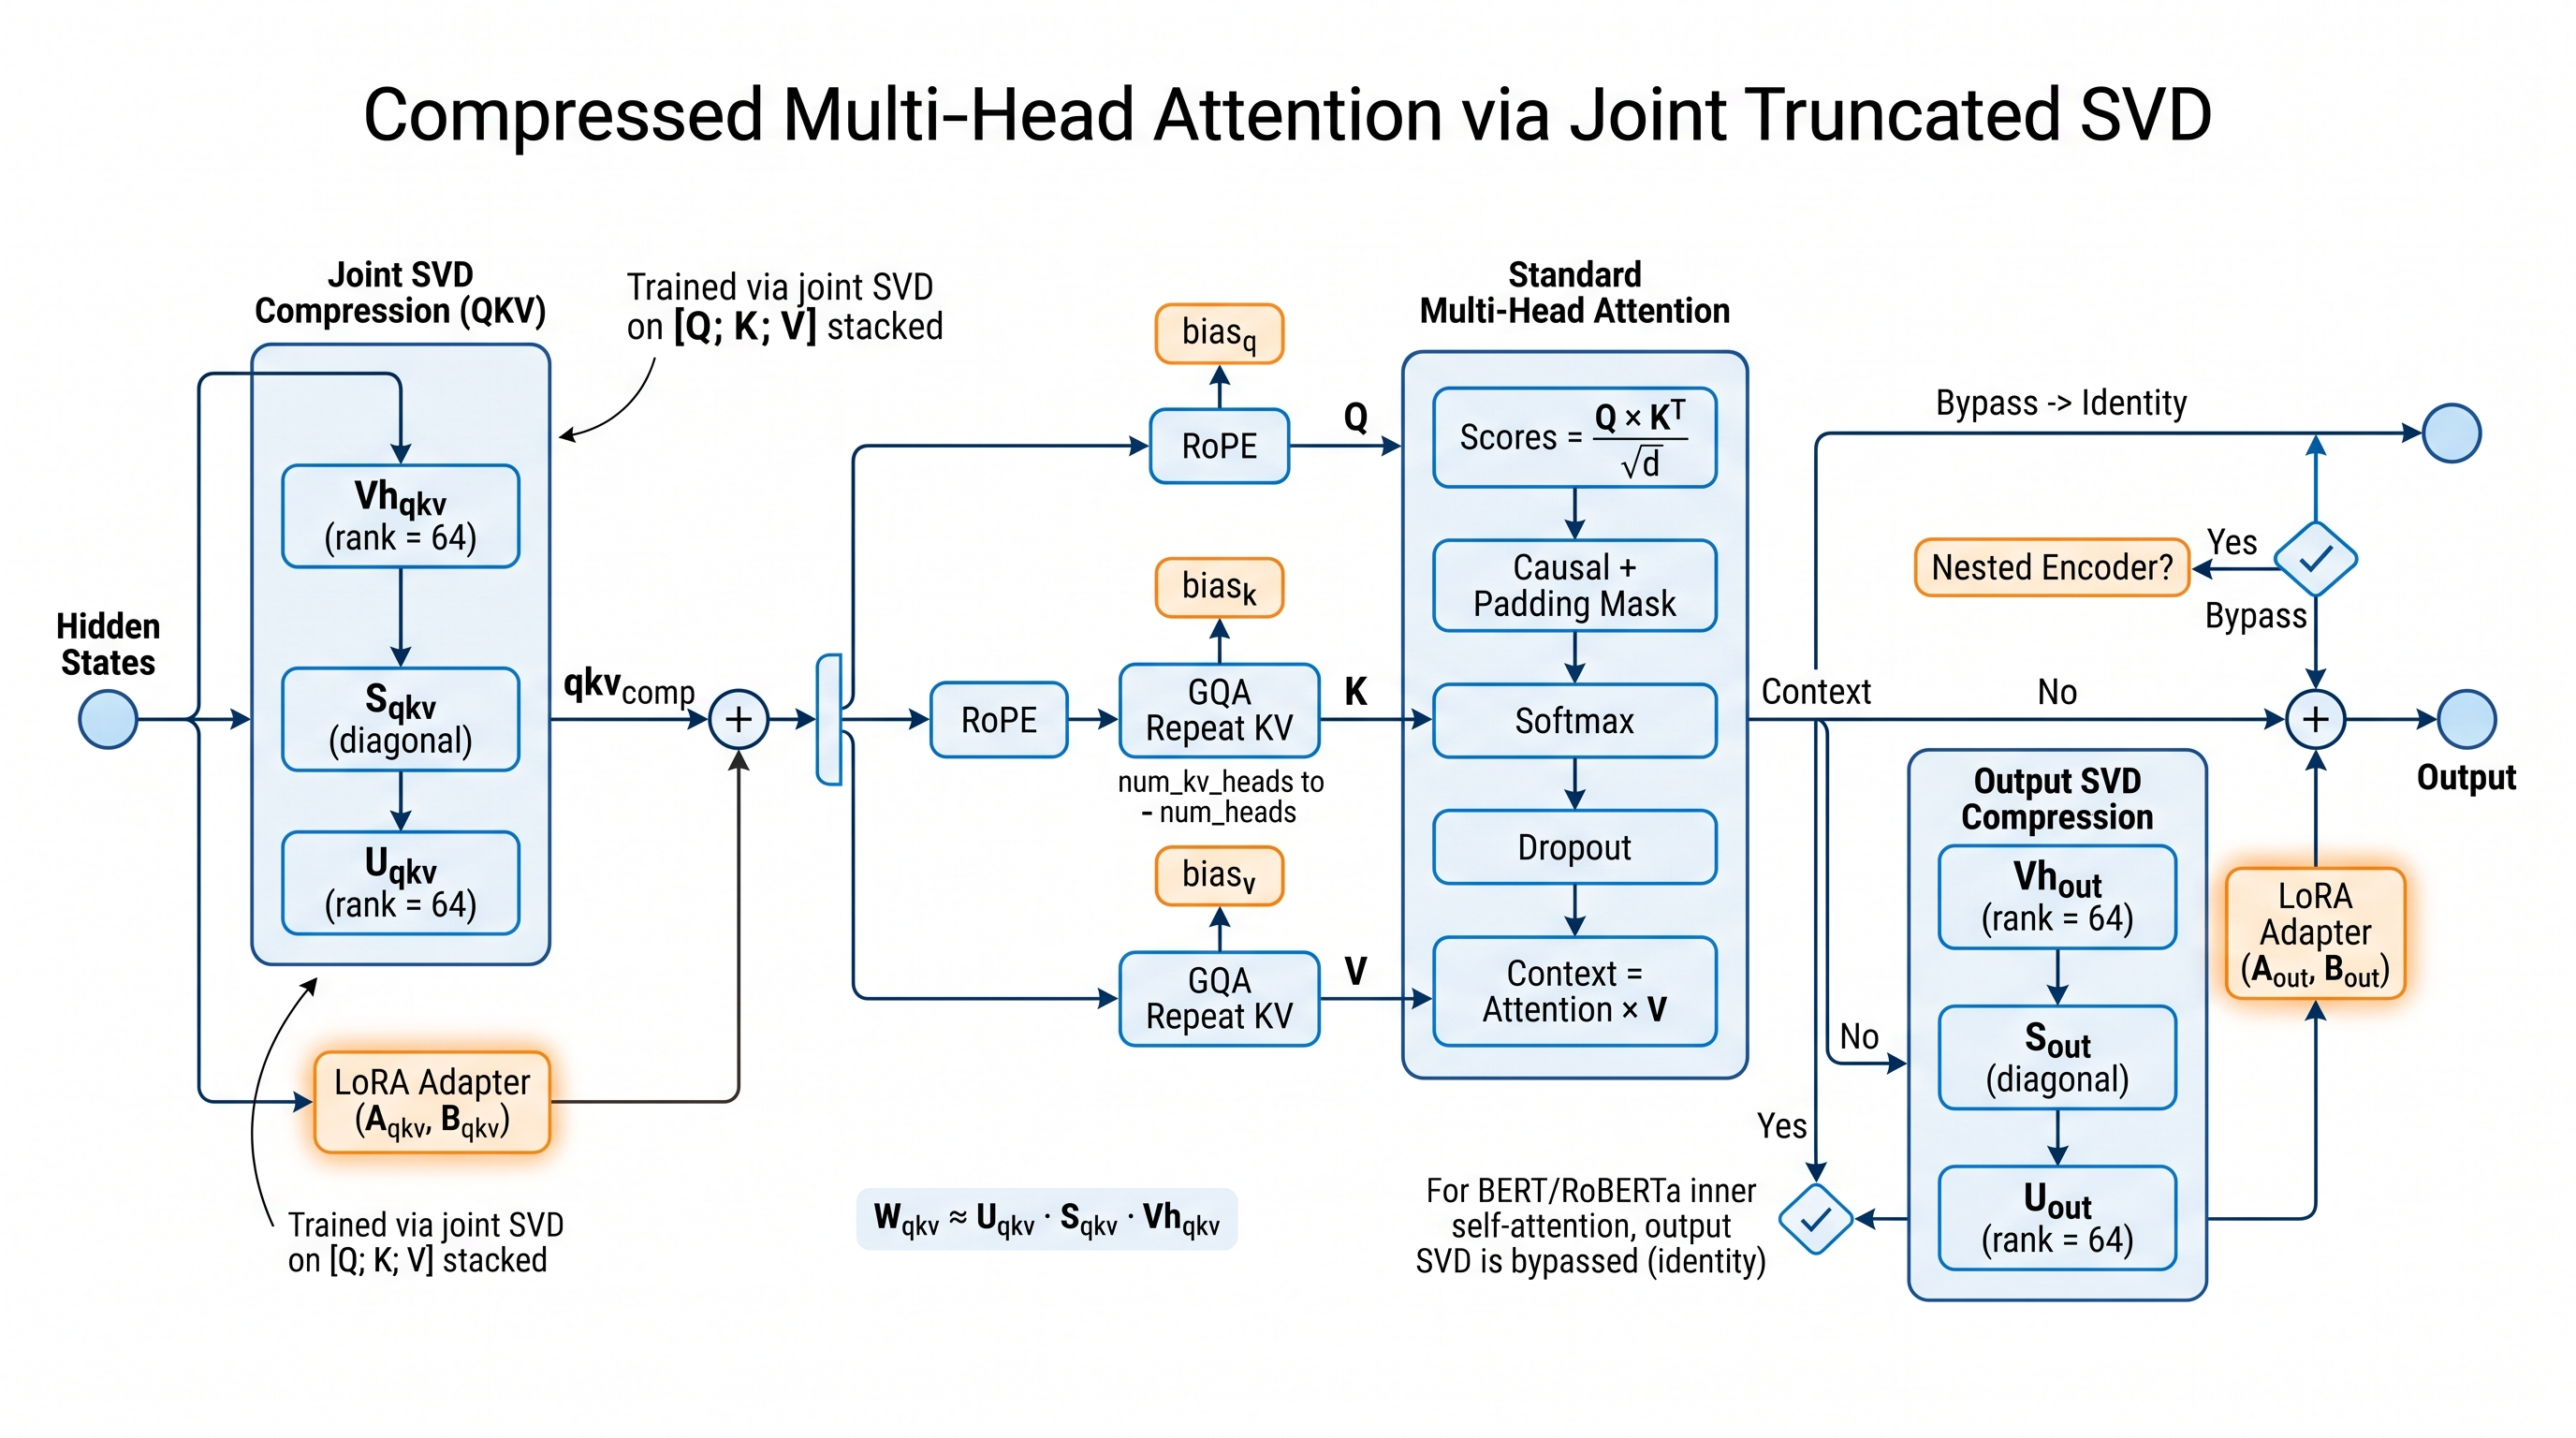
\includegraphics[width=\linewidth]{figures/architecture.jpeg}
\caption{High-level architectural diagram of compressed\_mha.}
\label{fig:arch\_compressed-mha}
\end{figure}

